\section{Results and Discussion}

For each run, I gather data such as loss, Q-values, episode reward and episode length; $\epsilon$ over time is also collected for debug purposes, but it is left out of the analysis because it is simply linearly annealed from $\epsilon_{\max}$ to $\epsilon_{\min}$ for each environment step for a total of \textit{max steps} $\times$ \textit{exploration fraction}, with no extra logic applied to it. Each model is trained on $20$ different fixed seeds (see \textbf{\nameref{section:appendix_c}}). I then interpolate the results of each run so that I can compute the mean of each episode. In order to denoise the mean score per episode, I also compute a smoothed version of the obtained line, a rolling average with $n = \frac{\text{number of episodes}}{10}$.

Despite being the most simple environment, none of the networks are able to learn to balance the pole in the \textit{CartPole} environment, and the \acrshort{tqn} fails to find a successful policy for \textit{Acrobot}. Supplementary analysis for these environments is relegated to the \textbf{\nameref{section:appendix_c}}. 

\begin{table}[H]
\label{table:results-LunarLander-v2}
\caption{Performance of the models tested across all the environments.}
\centering
\begin{tabular}{@{} r c c c c c c @{}}
\toprule
& \multicolumn{2}{c}{Acrobot-v1} & \multicolumn{2}{c}{CartPole-v1} & \multicolumn{2}{c}{LunarLander-v2} \\
\midrule
& $R_{\;mean}$ & $R_{\;best}$ & $R_{\;mean}$ & $R_{\;best}$ & $R_{\;mean}$ & $R_{\;best}$ \\
\midrule
DQN & \textbf{-91.99} & \textbf{-61} & \textbf{77.54} & 281.00 & \textbf{151.88} & 317.45 \\
TQN & -490.26 & -72 & 38.03 & \textbf{500} & 46.3 & \textbf{322.74} \\
\bottomrule
\end{tabular}
\end{table}

For the analysis, I take as a reference the \textit{LunarLander} environment, since it is the only one where both architectures converge. For the LunarLander environment, an episode is considered a valid solution if it scores $200$ points or more.

For the most relevant metrics I use \textbf{bootstrapping with stratified sampling} to compute the $95\%$ \textbf{confidence intervals}; the bootstrapping uses $50.000$ replications \footnote{The process of repeatedly sampling with replacement from the underlying data in order to create a simulated dataset.}; the sample efficiency curve normalizes the scores between $0$ and the target score $\tau = 200$.

\begin{figure}[!htbp]
\centering
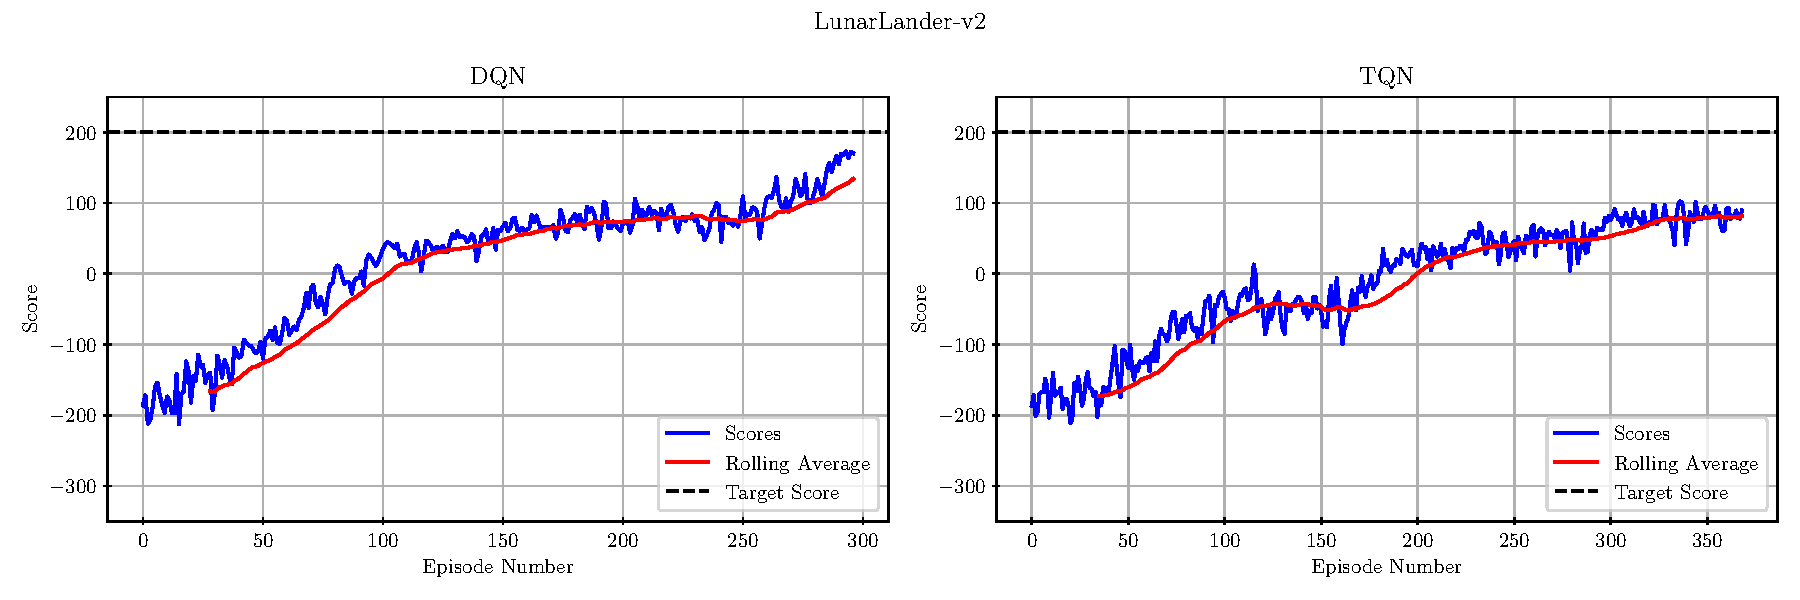
\includegraphics[width=\textwidth]{images/score-vs-episode_DQN-TQN_LunarLander-v2.pdf}
\caption{Each run has the same number of environment steps but, since the episode length is not fixed, the total number of episodes may differ.}
\label{fig:score-vs-episode-LunarLander-v2}
\end{figure}

In \textbf{Fig.}~\ref{fig:score-vs-episode-LunarLander-v2}, both sample efficiency curves have the shape of a logarithmic curve showing peak efficiency towards the end of the training and approaching the target score of $200$, but \acrshort{tqn} performs worse and has a higher variance. The new architecture shows convergence to the optimal policy over time, but from the plot it may seem that it is less efficient than the baseline. In reality, when I consider the the confidence intervals of the \textbf{\acrfull{iqm}}, the performance on the middle $50\%$ of the combined runs computed by removing the top and bottom $25\%$ of the runs \cite{rliable}, the probability of improvement shows that the \acrshort{tqn} performs better than the baseline (see \textbf{Fig.}~\ref{fig:sample-efficiency-LunarLander-v2}). The \textbf{probability of improvement} is a metric that shows how likely it is for $X$ to outperform $Y$ on a randomly selected task, where 

\begin{equation}
P(X > Y) = \frac{1}{M} \sum^M_{m=1} P(X_m > Y_m),
\label{eq:probability_of_improvement}
\end{equation}

with $P(X_m > Y_m)$ the probability of $X$ being better than $Y$ at task $m$ \cite{rliable}.

In this case, $P(\acrshort{dqn} > \acrshort{tqn}) = 0.48$, which is equivalent to say $P(\acrshort{tqn} > \acrshort{dqn}) = 0.52$, meaning that, given a random task, the \acrlong{tqn} gets a better reward than the baseline $52\%$ of the time.

\begin{figure}[!htbp]
\centering
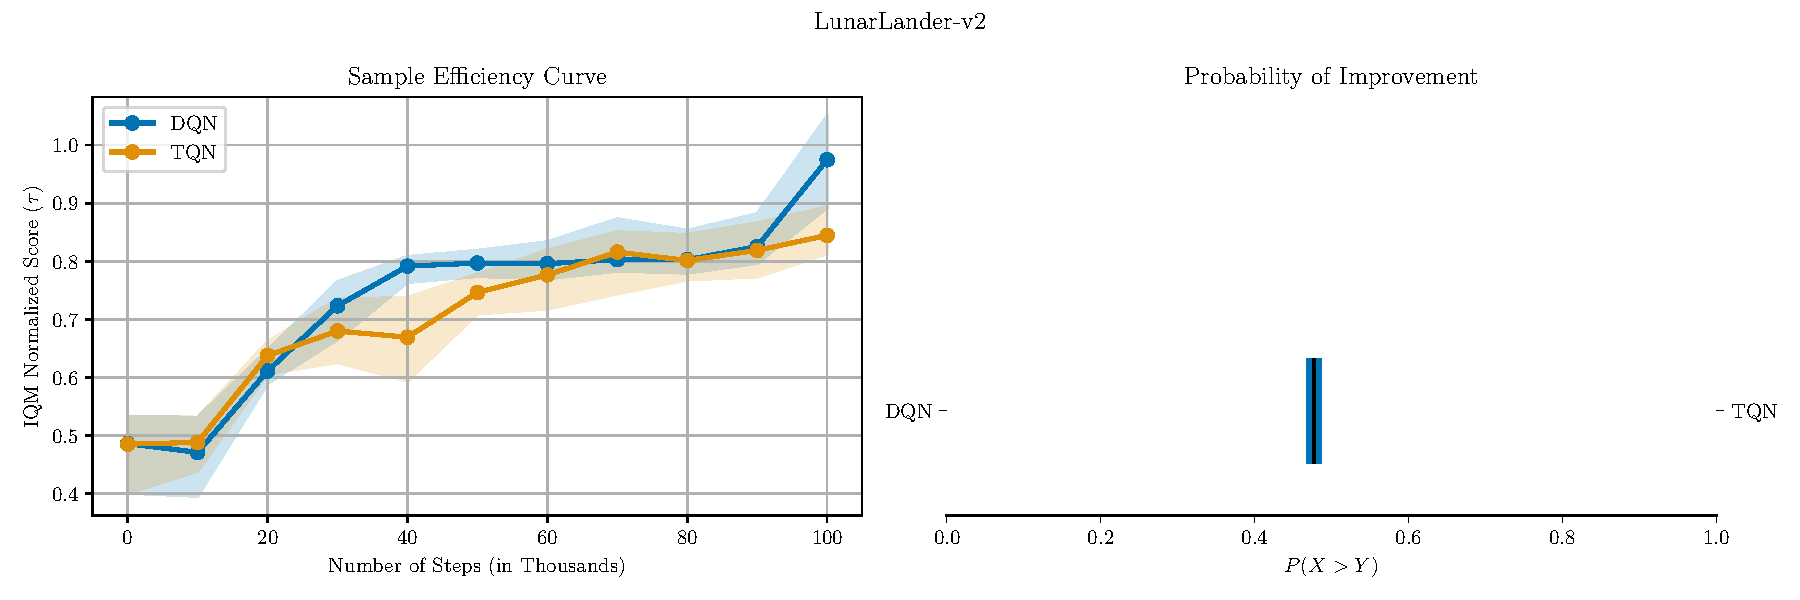
\includegraphics[width=\textwidth]{images/sample-efficiency-probability-improvement_DQN-TQN_LunarLander-v2.pdf}
\caption{On the left, sample efficiency of agents as a function of number of steps measured via \acrshort{iqm} scores. Shaded regions show pointwise 95\% percentile stratified bootstrap CIs, as suggested by \cite{rliable}. On the right, the probability of improvement.}
\label{fig:sample-efficiency-LunarLander-v2}
\end{figure}

To check whether each model has over-confident Q-values, I average the results of $400$ test runs for each architecture ($20$ models, $1$ for each seed, play environments tested with all the seeds). For a consistent range of comparison, both the rewards and Q-values gathered this way are normalized between $-1$ and $1$.

\begin{figure}[!htbp]
\centering
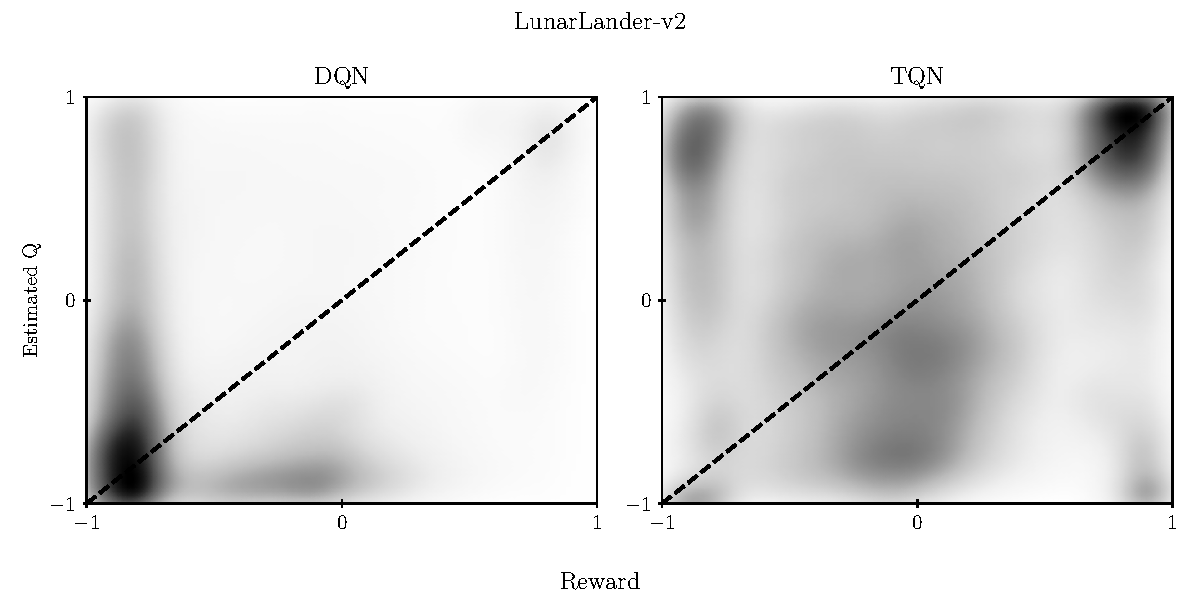
\includegraphics[width=\textwidth]{images/q-vs-reward_LunarLander-v2.pdf}
\caption{Density plot of the estimated Q-values versus environment step rewards sampled from $400$ episodes.}
\label{fig:q-vs-reward-LunarLander-v2}
\end{figure}

Despite the Q-values represent the overall confidence of the network while the step rewards are only an immediate feedback, it is still useful to visualize their relationship to better understand the behavior of the two architectures. As the rewards increase, the Q-values should also increase. Ideally, in \textbf{Fig.}~\ref{fig:q-vs-reward-LunarLander-v2}, the density should be aligned with the major diagonal. This would mean that Q-values estimates are well-aligned with the rewards each agent receives.

I can observe that, while both models present fluctuation, \acrshort{dqn} is more robust and it takes a more conservative approach; it is the most ``pessimistic" when it receives low rewards. The \acrshort{tqn} architecture instead is over-confident in its estimates and, although the model is most confident when it receives the highest rewards, as expected, it also shows a high degree of confidence when it receives the lowest rewards.

\begin{figure}[!htbp]
\centering
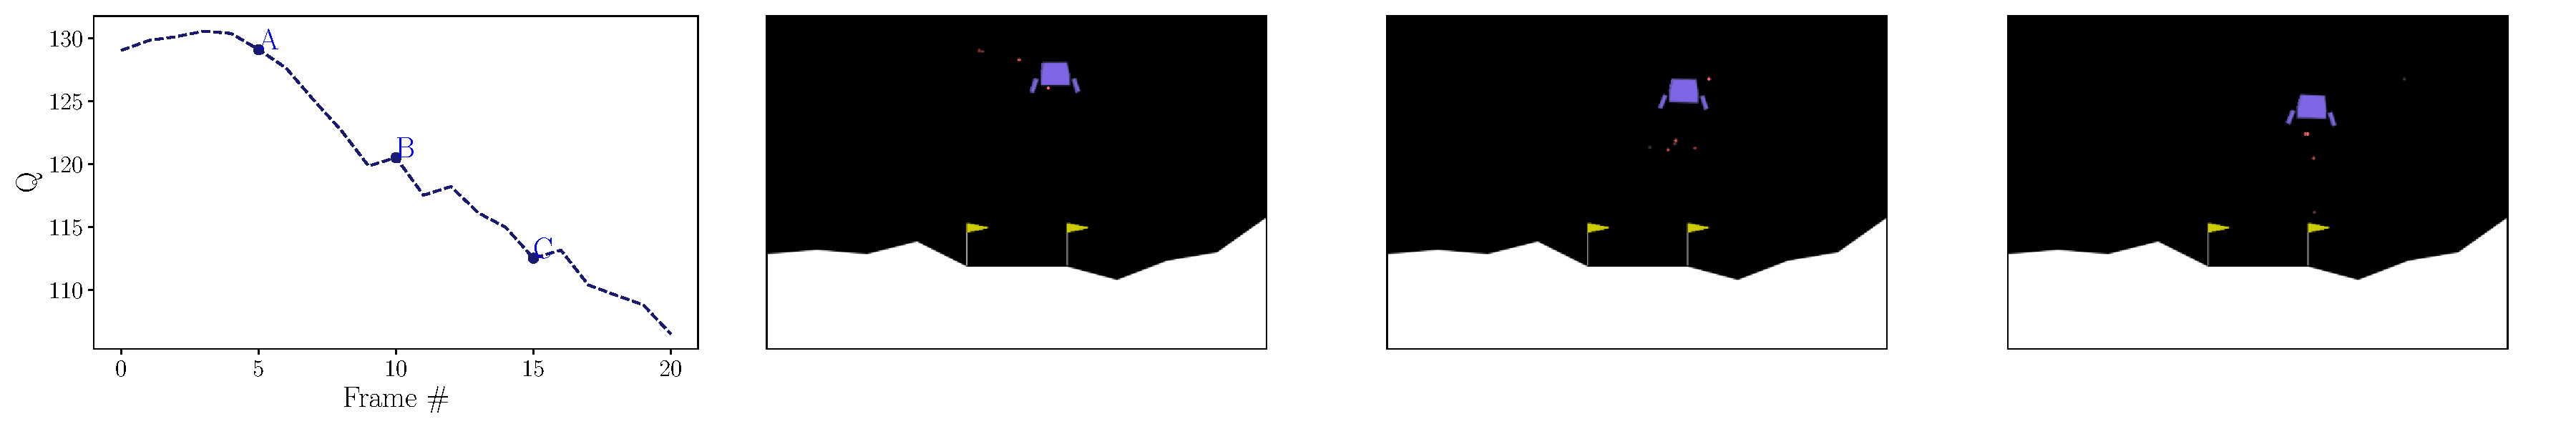
\includegraphics[width=\textwidth]{images/q-vs-frame_DQN_LunarLander-v2.pdf}
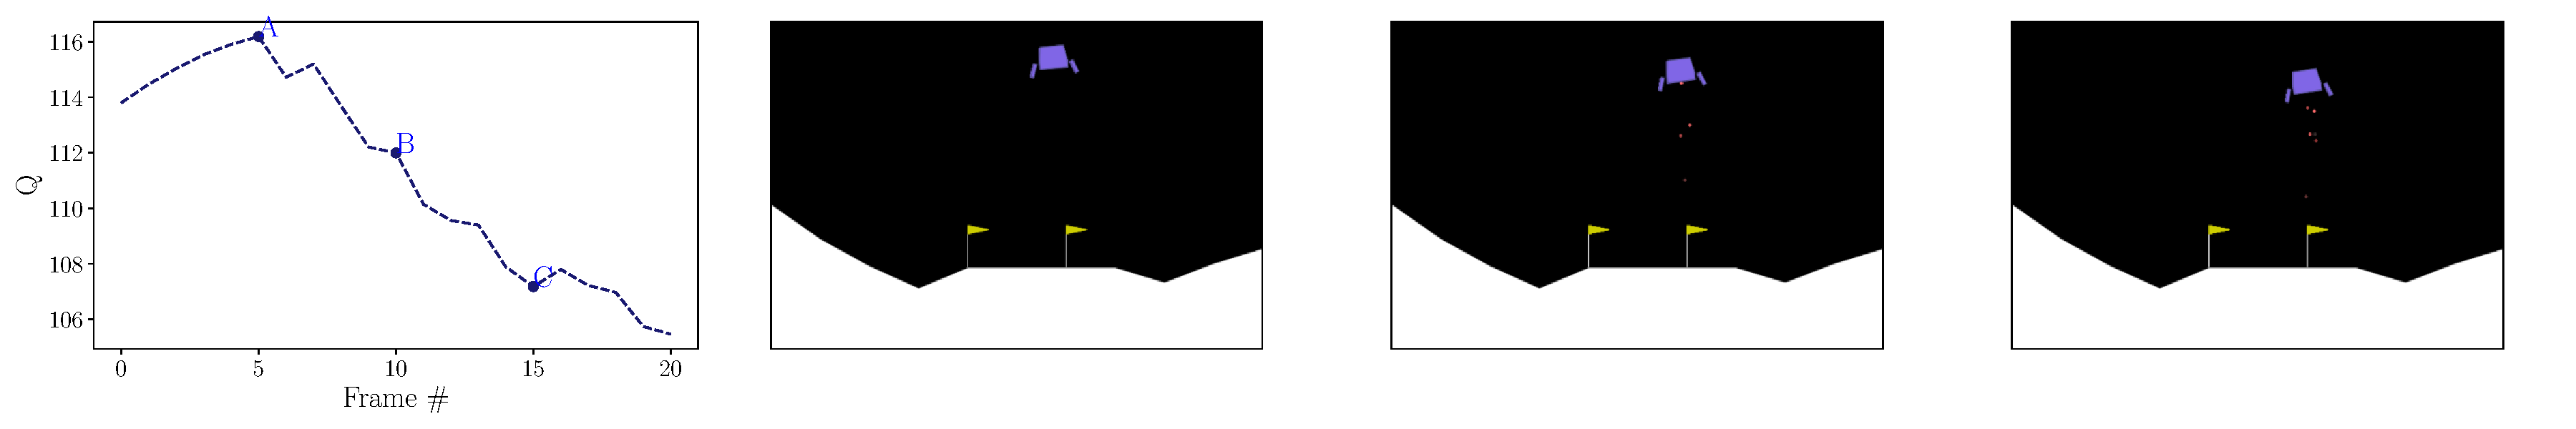
\includegraphics[width=\textwidth]{images/q-vs-frame_TQN_LunarLander-v2.pdf}
\caption{On the left, the predicted Q-values for a portion of a LunarLander episode. The three screenshots on the right correspond to the frames labeled by A, B, and C. The first row is from the \acrlong{dqn} and the second one from the \acrlong{tqn}.}
\label{fig:q-vs-screenshot-TQN-LunarLander-v2}
\end{figure}

Despite using a target network to dampen its confidence, \acrshort{tqn} is still prone to over-estimating Q-values. The over-confidence in the predictions matches what I show in \textbf{Fig.}~\ref{fig:q-vs-reward-LunarLander-v2}; the step of the loss function indicates that \acrshort{tqn} has learned steadily during training, but it has not fully converged yet.

\begin{figure}[!htbp]
\centering
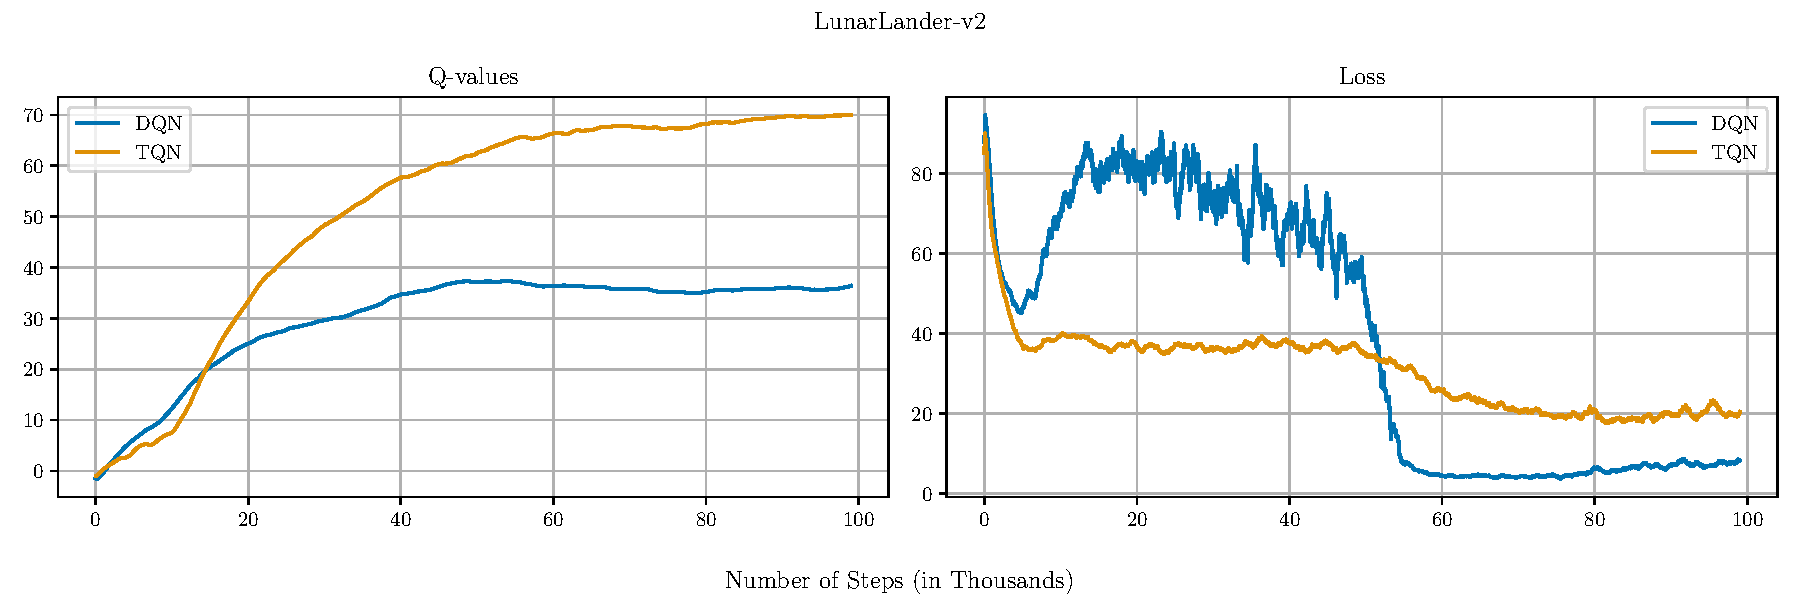
\includegraphics[width=\textwidth]{images/q-vs-loss_DQN-TQN_LunarLander-v2.pdf}
\caption{Q-values over time and loss over time. \acrshort{tqn} is over-confident and converges more slowly.}
\label{fig:q-vs-loss-LunarLander-v2}
\end{figure}

The last metrics (Fig.~\ref{fig:statistics-LunarLander-v2}) are again computed by normalizing the scores between $0$ and $\tau = 200$, the target score for which an episode of the LunarLander environment is considered successful (see \nameref{subsubsec:lunar_lander}). Albeit the magnitude is very small ($10^{-2}$), the \acrlong{tqn} is able to beat the baseline \acrshort{dqn} baseline. Large confidence intervals for the \textbf{median} mean that there are a few high performing tasks skewing the results and, to compensate for it, I choose the \acrshort{iqm}, explained above, as a better indicator of the performance \cite{rliable}. The \acrshort{iqm} is more robust than the mean to statistical outliers and, thanks to the smaller confidence intervals, it is able to detect improvements with fewer runs \cite{rliable}. As opposed to the probability of improvement, both the \acrshort{iqm} and the optimality gap that follows take into account the size of improvement.

\begin{figure}[!htbp]
\centering
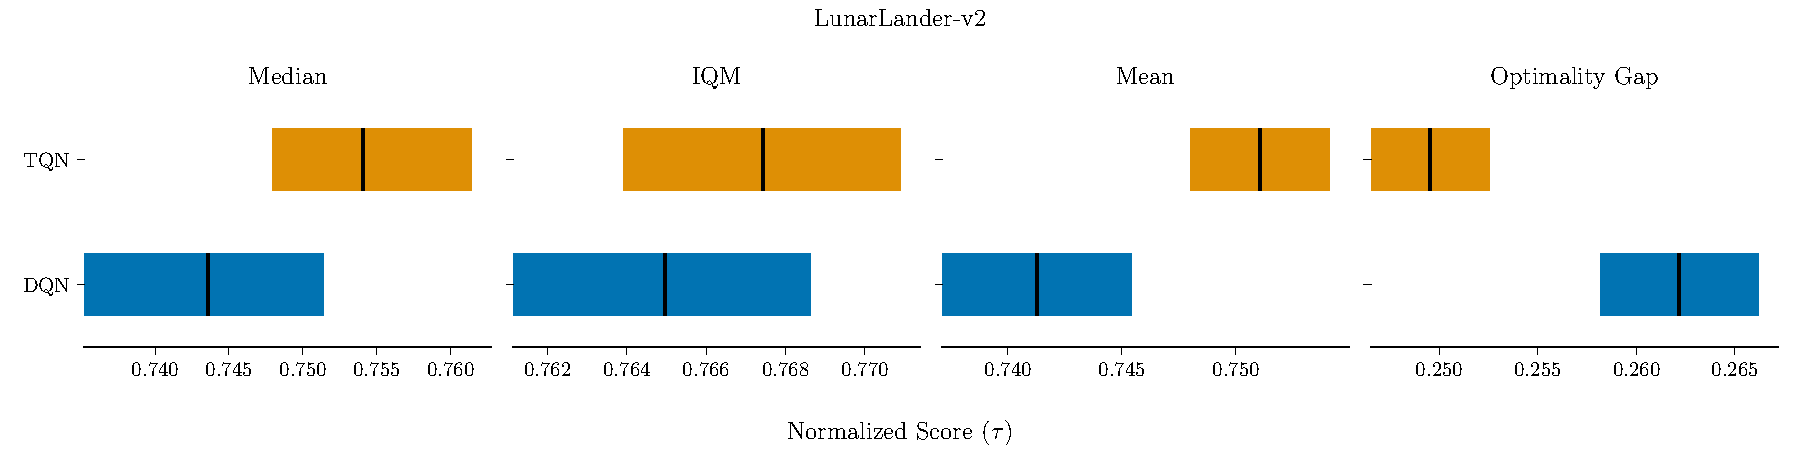
\includegraphics[width=\textwidth]{images/statistics_DQN-TQN_LunarLander-v2.pdf}
\caption{Aggregate metrics with 95\% confidence intervals.}
\label{fig:statistics-LunarLander-v2}
\end{figure}

Finally, a more robust alternative to the mean is the \textbf{optimality gap}, which is the amount by which the models fail to meet the target score $\tau$. The optimality gap assumes that scores above the threshold are less important than the rest. In this case a higher value corresponds to worse performance, and the results in \textbf{Fig.}~\ref{fig:statistics-LunarLander-v2} once again confirm that the novel architecture performs indeed better than the baseline.
